

\subsection{Software}

\subsubsection{Architecture}
For the architecture of the test software, it was decided to adopt a modular approach with separate classes for each test and measurement instrument. This architecture facilitates easy extension of the software with new instruments and tests. Additionally, it allows looping over different tests without the need to initialize and close measurement instruments every time they are used. For data storage, the decision was made to employ a database, as it offers a convenient way to store and analyze data afterward. Thereby SQLite was chosen as the database solution due to its lightweight nature and ease of use, requiring no server to be running. The database was structured with the following columns:
\begin{itemize}
    \item \textbf{Id}: The unique identifier for each measurement.
    \item \textbf{chip\_id}: The identifier for the chip that was measured.
    \item \textbf{measurement\_type}: The type of measurement performed.
    \item \textbf{parameter1}: The first parameter used for the test, such as the input voltage applied.
    \item \textbf{parameter2}: The second parameter used for the test, such as the load applied to the output.
    \item \textbf{temperature}: The temperature of the chip during the measurement.
    \item \textbf{data}: The measured data.
    \item \textbf{measurement\_result}: The result of the measurement, if applicable.
    \item \textbf{Timestamp}: The timestamp of the measurement.
\end{itemize}

\subsubsection{Test Software Language}
The test software was implemented using Python. Python is a high-level programming language widely utilized in the scientific community and increasingly in testing due to its ease of learning and the availability of drivers for nearly every measurement instrument\cite{Wikipedia:Python}. Additionally, one of the authors had prior experience in writing test scripts in Python for chip verification and validation, enabling the initiation of test writing without a significant investment in learning a new programming language and environment.

\subsubsection{Test Software Implementation}
Prior to commencing the test software development, the various tests to be performed were determined, aiming to align with those conducted in simulations. These included:
\begin{itemize}
    \item Startup behavior with reset disabled.
    \item Startup behavior with active reset and subsequently disabled reset.
    \item Load step response with load variations of 10mA, 100mA, and 200mA.
    \item Output response to stepped input voltage changes.
    \item Turn-off and turn-on behavior with brief reset enablement.
    \item SPI test to mux out the wanted analog/digital signal, change the clock frequency, and read back the register values.
\end{itemize}

\subsubsection{Test Setup}
The primary test setup utilized the PXI system from National Instruments (NI). This system integrates various measurement instruments into a single unit and serves as the computer running the Python code. Consequently, there are no delays due to additional wires between the computer and measurement instruments. Moreover, synchronized triggers are available on this measurement system, eliminating the need for trigger wiring between instruments. This advantage reduces setup complexity and wiring requirements. The specific PXI system employed was the PXI model \glqq{}NI PXIe-8881\grqq{}, equipped with the following modules:

\begin{itemize}
    \item \textbf{PXIe-4141}: This is a SMU (Source Measurement Unit) which can be used to apply the input voltage to the chip.
    \item \textbf{E3631A}: This is a power supply which can be used to apply the input voltage to the chip.
    \item \textbf{PXI-5142}: This is a two channel oscilloscope used to measure the output and input voltage of the chip.
    \item \textbf{PXI-5163}: This is a two channel oscilloscope used to measure the output and input current of the chip.
    \item \textbf{TP04300}: This is the thermostreamer used to control the temperature of the chip.
    \item \textbf{PXI-6363}: This is a GPIO controller used to control the reset of the chip and the different load resistors.
    \item \textbf{NGE-100}: This is a power supply to provide the power for the test circuit.
    \item \textbf{FTDI C232HM-DDHSL-0}: This is a USB to SPI converter used to communicate with the chip.
\end{itemize}

An overview of all the instruments can be seen in Figure \autoref{fig:overview}. More details about the hardware can also be found in the \href{https://github.com/gstei/asic_validation/}{git repository}\footnote{https://github.com/gstei/asic\_validation.git} where test was written.

\begin{figure}[h]
    \centering
    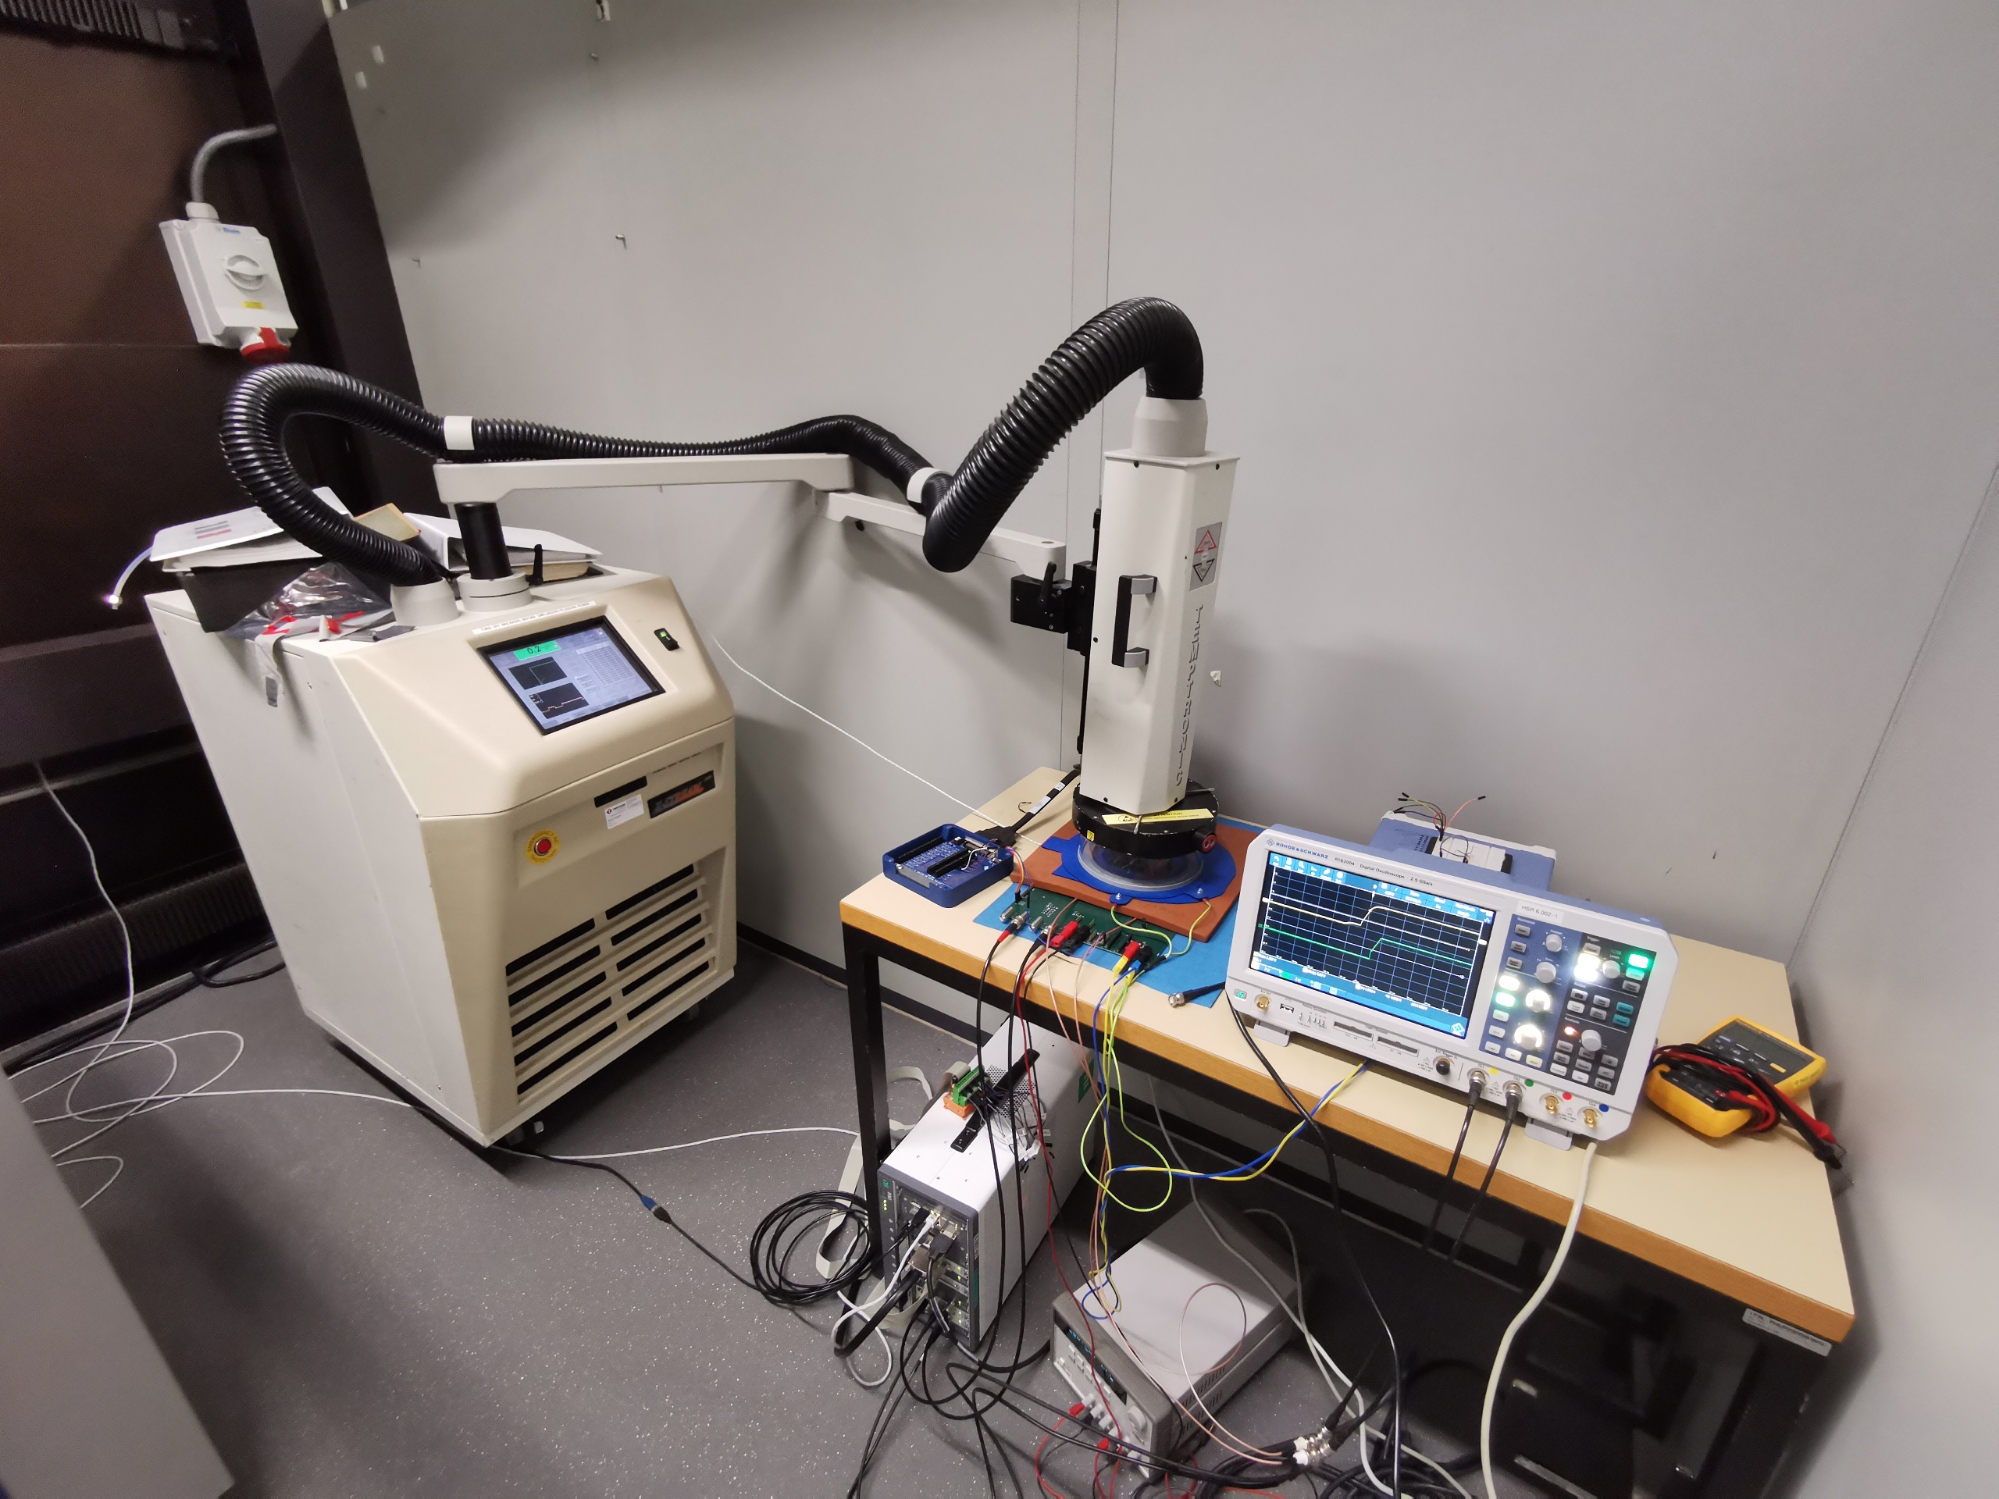
\includegraphics[width=0.8\textwidth]{../ASIC-DESIGN-2/images/02_test_setup/01_overview.jpg}
    \caption{Overview of the test setup}
    \label{fig:overview}
\end{figure}

\subsubsection{Github}
The test software was written using Git as its version control system, with the repository being hosted on GitHub. This choice was driven by GitHub's widespread adoption and its seamless integration for collaborative code sharing among team members. Furthermore, Git's robust features allow for efficient tracking of changes and management of various software versions. The repository can be found at \href{https://github.com/gstei/asic_validation.git}{the following link}\footnote{https://github.com/gstei/asic\_validation.git}. Furthermore the repository uses github actions to automatically run tests on every push to the repository. This ensures that the code is written in a nice way according to the PEP8 standard and that the tests are most probably running without any errors, for that \href{par:Flake8}{flake8} and \href{par:Pylint}{pylint} were used as linter and integrated in the github workflow.

\paragraph{Pylint}
\label{par:Pylint}
Pylint is a static code analysis tool for Python, adhering to the style guidelines outlined in PEP 8. It checks various aspects of Python code, including line length, variable naming conventions, and interface implementation consistency. Pylint is similar to Pychecker and Pyflakes but offers additional features such as generating UML diagrams using the Pyreverse module. It can be used independently or integrated into various IDEs and editors like Eclipse with PyDev, Spyder, Visual Studio Code, Atom, GNU Emacs, and Vim\cite{Wikipedia:Pylint}.

\paragraph{Flake8}
\label{Par:Flake8}
Flake8 is a Python linting tool that scans Python codebases for errors, style inconsistencies, and complexity. It consists of three underlying tools: PyFlakes for error checking, McCabe for complexity analysis, and pycodestyle for style conformity with PEP8 guidelines. Flake8 stands out due to its extensive plugin ecosystem, allowing users to augment its capabilities and address a wide range of issues and concerns in Python code\cite{flake8}.


\subsubsection{SPI Interface}
\label{subsubsec:SPI}
The registers of the chip can be controlled over a SPI interface, therefore a SPI Master was needed.
It was decided to implemented the SPI master using the FTDI C232HM-DDHSL-0 USB to SPI converter. The FTDI chip was chosen due to its ease of use and the availability of drivers for Python. But it finally turned out that the SPI mode 1 which was implemented on the chip does not exactly correspond to SPI mode 1 implemented on the FTDI Chip. On the FTDI Chip the CS and the first SPI clock edge are turned on on the same time, but on the test bench used in the simulation to verify the digital part of the chip this was not the case and due to its implementation the finite state machine only works when the CS is turned on before the first clock edge as it is also visible in \autoref{fig:spi_modes} (CPOL=0, CPHA=1). Therefore a custom driver was implemented in software which only works at 1kHz instead of 500kHz, but since one only needs to write eight different register this does not really matter. Since the human counterpart does not see the difference. Nevertheless for further projects we would recommend to have a look at the test instruments already when designing the chip to avoid such problems. Nevertheless the SPI interface should work with a normal micro controller which uses the SPI standard as as it can be seen in \autoref{fig:spi_modes} where the CS is turned on before the first clock edge. Nevertheless there are some special implementations of the SPI as in the FTDI C232HM-DDHSL-0 which should have been covered as well during the design.
\begin{figure}[h]
    \centering
    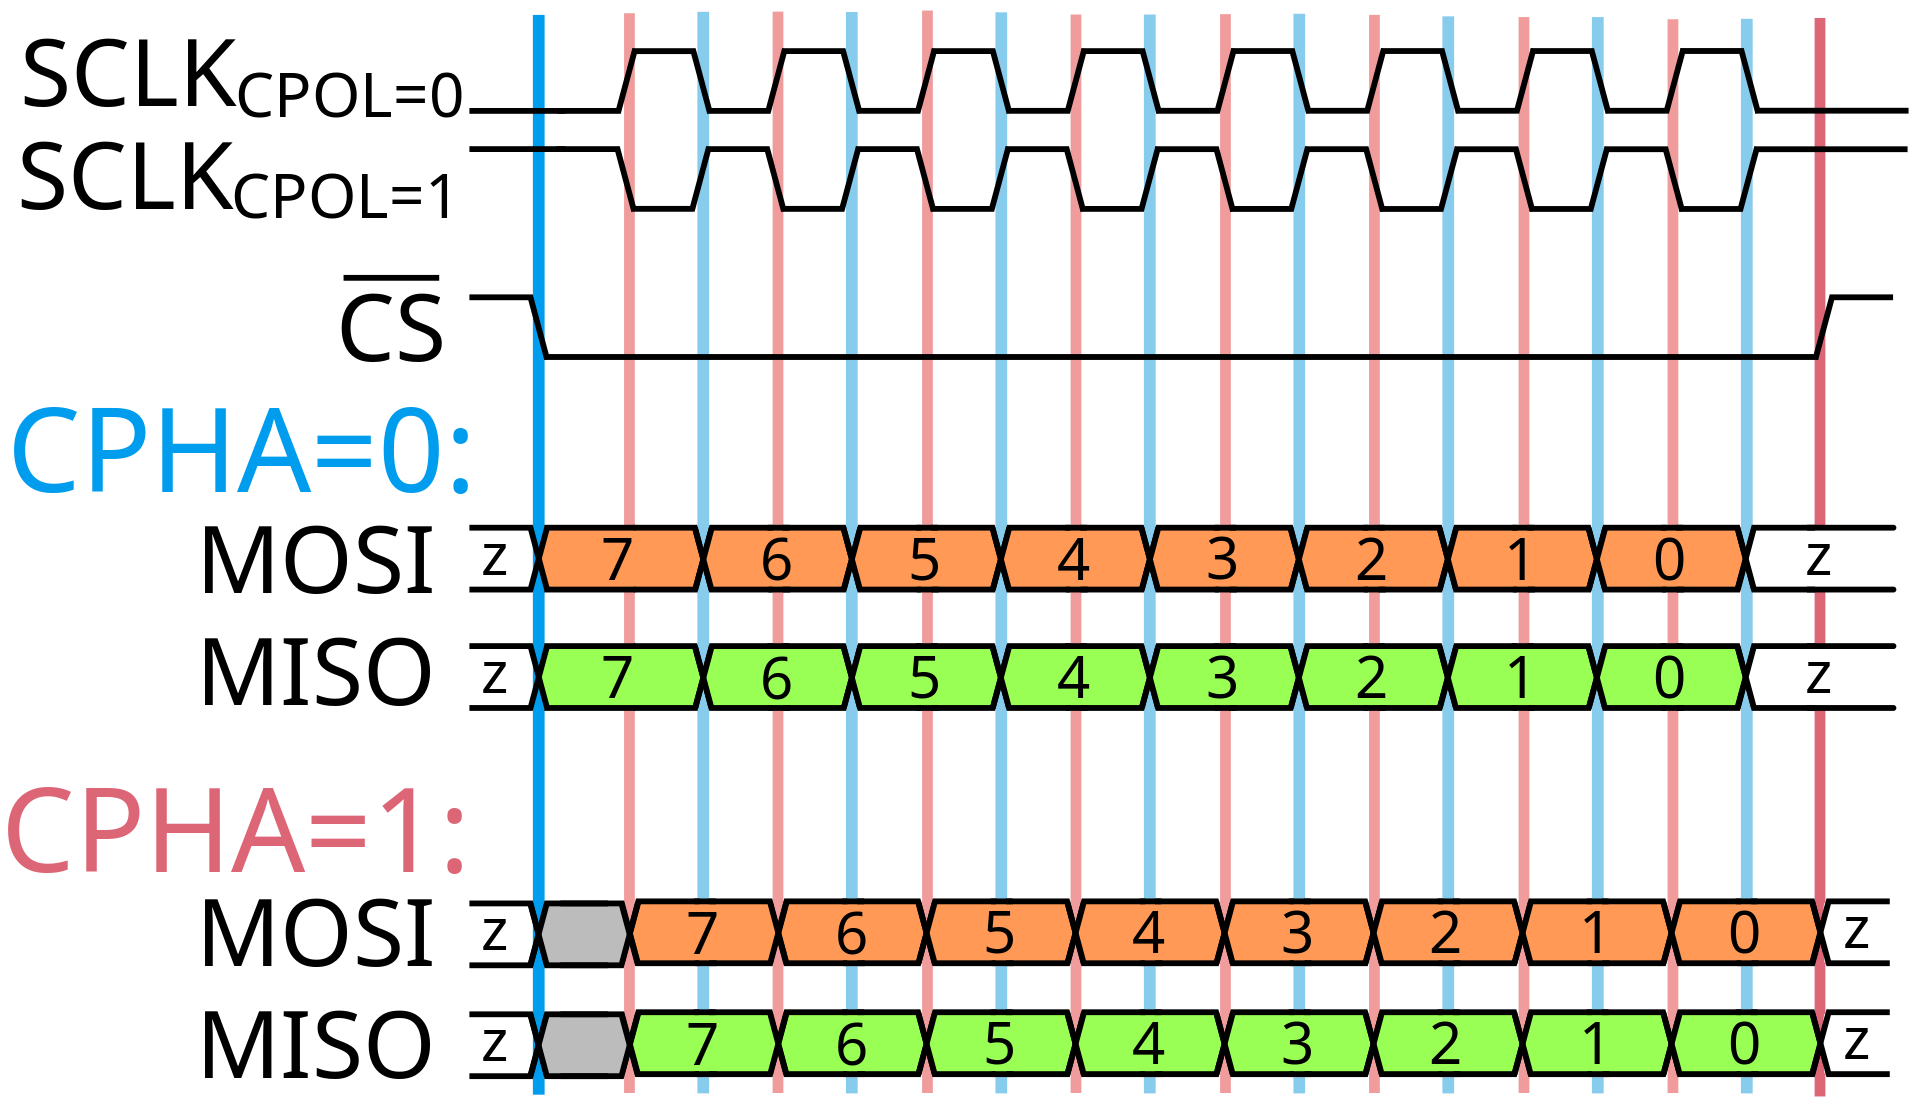
\includegraphics[width=0.8\textwidth]{../ASIC-DESIGN-2/images/04_spi/SPI_timing_diagram_CS.svg.png}
    \caption{SPI Modes \cite{Wikipedia:SPI}}
    \label{fig:spi_modes}
\end{figure}
\subsubsection{Conclusion}
In retrospective one can say that it was a very good decision to spend quite some time in the software architecture in the beginning of the project and to use a database. Since it turned out that once it is clear what and how something has to be implemented the software can be written quite fast and with the code checker in the background also with a reasonable quality, this for example allowed to add the thermostreamer to the tests within two hours without any issues and all measurement results were available in the database. Nevertheless it also turned out that when the chip does not behave as expected the test script is not useful at all. Due to that the automated tests only worked with the TI chip, but not with our chip since we had startup problems on our chip which caused that the whole automated test could not be executed since the chip started not correctly as also mentioned in 
\autoref{subsubsec:cur_mes_inac}.


